% $Header$

\documentclass[aspectratio=169]{beamer}

\mode<presentation>
{
  \usetheme{default}
  % or ...

  \usecolortheme{rose}
  \useinnertheme{rectangles}
  \useoutertheme[hooks]{tree}
  \setbeamercovered{transparent}
  % or whatever (possibly just delete it)
}


\usepackage{bm}
\usepackage[english]{babel}
\usepackage{multicol}
% or whatever
\usepackage{tikz}
\usepackage[latin1]{inputenc}
% or whatever
\usepackage{graphicx}
\usepackage[super]{nth}
\usepackage{amsmath}
\usepackage[T1]{fontenc}
% Or whatever. Note that the encoding and the font should match. If T1
% does not look nice, try deleting the line with the fontenc.


\title % (optional, use only with long paper titles)
{ CS/Math: Mathematics for Machine Learning}

\subtitle{\Large \textit {Cloud Point Reduction via Matrix Methods}}
\author[Hamza, Hussain, Mir] % (optional, use only with lots of authors)
{Ali Hamza \and Affan Mir \and Fasih Hussain}

\institute{Habib University} % (optional, but mostly needed)
\date{\today} % (optional, should be abbreviation of conference name)

\pgfdeclareimage[height=1cm]{university-logo}{images/logo.jpg}
\logo{\pgfuseimage{university-logo}}



\AtBeginSection[]{
  \begin{frame}
  \vfill
  \centering
  \begin{beamercolorbox}[sep=8pt,center,shadow=true,rounded=true]{title}
     \usebeamerfont{title}\Huge\insertsectionhead\par%
  \end{beamercolorbox}
  \vfill
  \end{frame}
}


\begin{document}

\begin{frame}
  \titlepage
  \begin{center}
      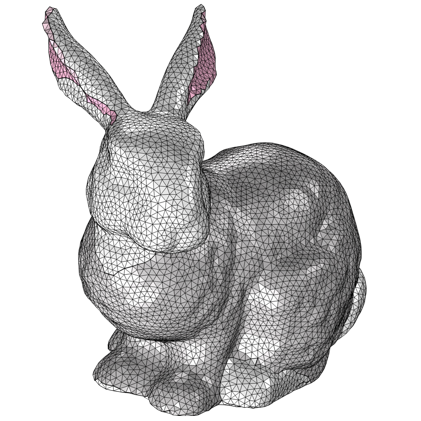
\includegraphics[scale=0.2]{images/img.png}
  \end{center}
\end{frame}
\setcounter{tocdepth}{1}
\begin{frame}{Outline}

    \tableofcontents
\end{frame}

%%%%%%%%%%% SECTION 1%%%%%%%%%%%%%%%
% \section{Introduction}

% \subsection{Problem Statement}
% \begin{frame}
%   \frametitle{Problem Statement}
% \end{frame}

% \subsection{Proposed Solutions}
% \begin{frame}
%   \frametitle{Proposed Solutions}
% \end{frame}

\section{Compression via SVD}

\subsection{General Idea}
\begin{frame}{General Idea}
  \begin{center}
      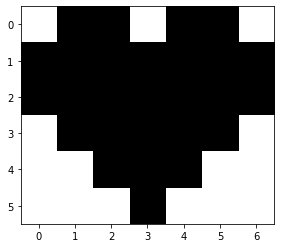
\includegraphics[scale=0.5]{images/heart1.png}
  \end{center}
\end{frame}
\begin{frame}{General Idea}
    \begin{table}[h]
\centering
\begin{tabular}{|l|l|l|l|l|l|l|}
\hline
    0 & 1 & 1 & 0 & 1 & 1 & 0\\ \hline
    1 & 1 & 1 & 1 & 1 & 1 & 1\\ \hline
    1 & 1 & 1 & 1 & 1 & 1 & 1\\ \hline
    0 & 1 & 1 & 1 & 1 & 1 & 0\\ \hline
    0 & 0 & 1 & 1 & 1 & 0 & 0\\ \hline
    0 & 0 & 0 & 1 & 0 & 0 & 0\\ \hline
\end{tabular}
\end{table}
\end{frame}

\begin{frame}{General Idea}
\[\scalebox{1.8}{$\begin{bmatrix} A_1 \end{bmatrix} +  \begin{bmatrix} A_2 \end{bmatrix} +  \begin{bmatrix} A_3 \end{bmatrix} +  \begin{bmatrix} A_4 \end{bmatrix} +  \begin{bmatrix} A_5 \end{bmatrix} +  \begin{bmatrix} A_6 \end{bmatrix} $}\]
\end{frame}
\begin{frame}
\frametitle{General Idea}
  \begin{center}
  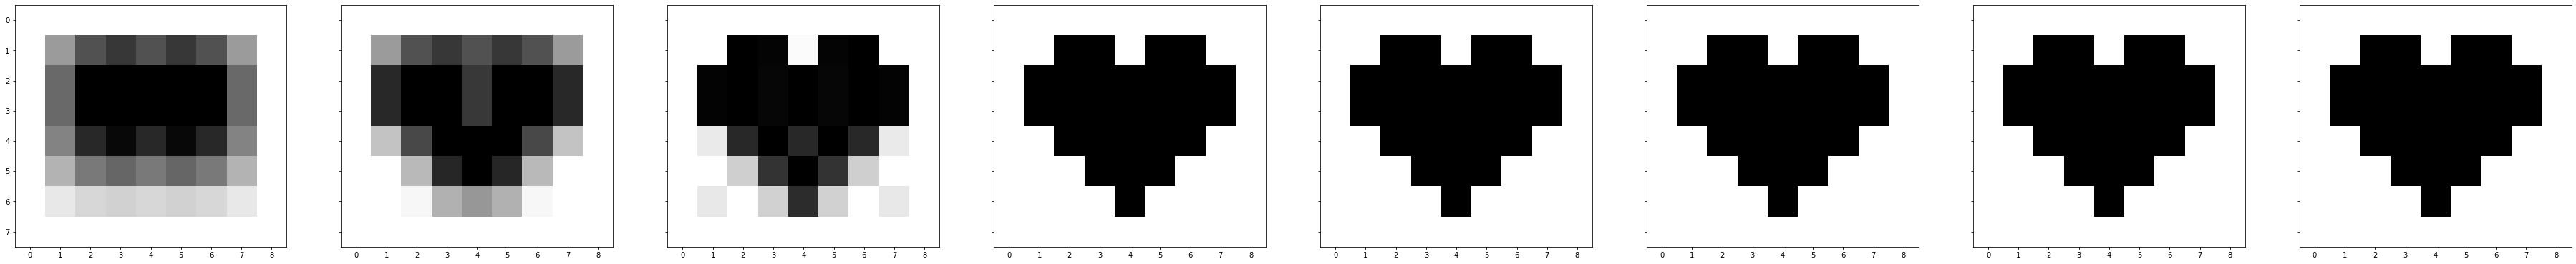
\includegraphics[scale = 0.1]{images/heart.png}
  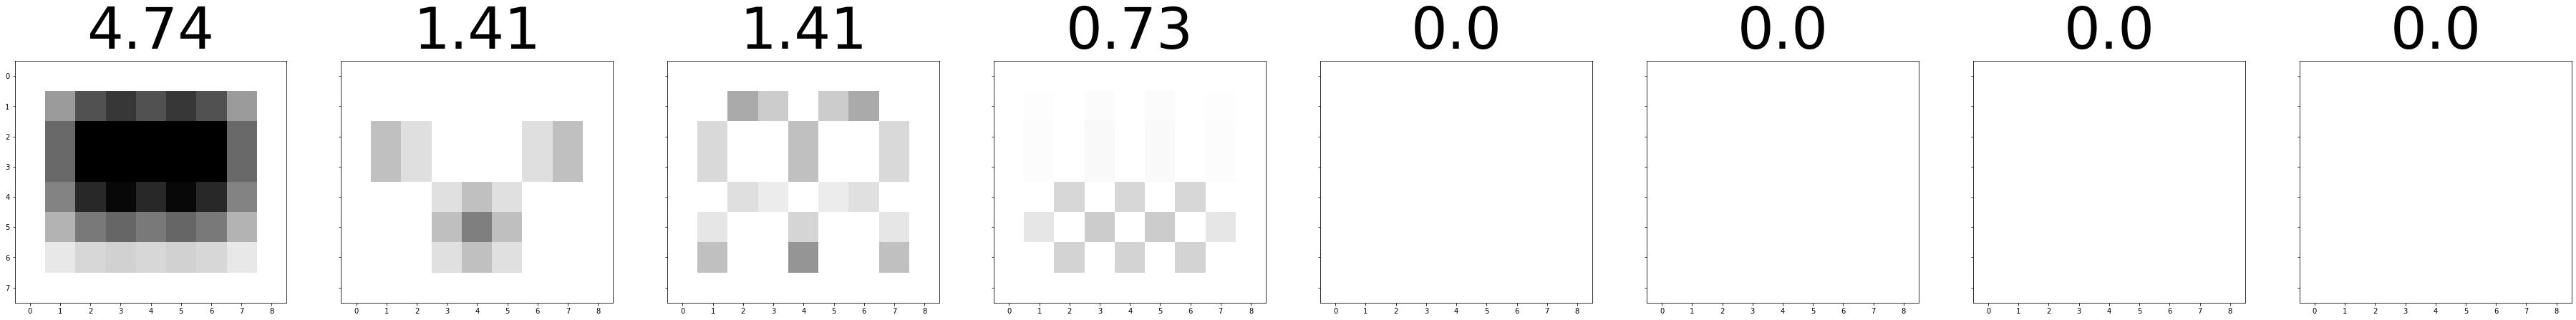
\includegraphics[scale = 0.1]{images/svdheart.png}
  \end{center}
\end{frame}

\begin{frame}{General Idea}
    \begin{center}
        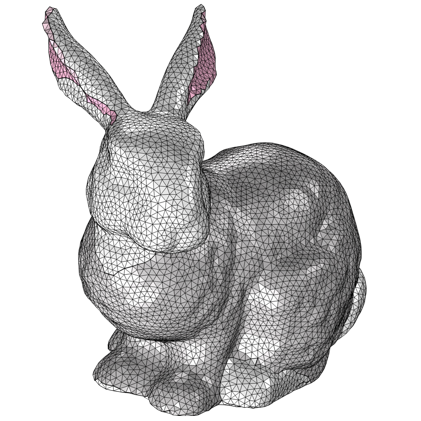
\includegraphics[scale = 0.4]{images/img.png}
    \end{center}
\end{frame}
\begin{frame}{General Idea}
\begin{center}
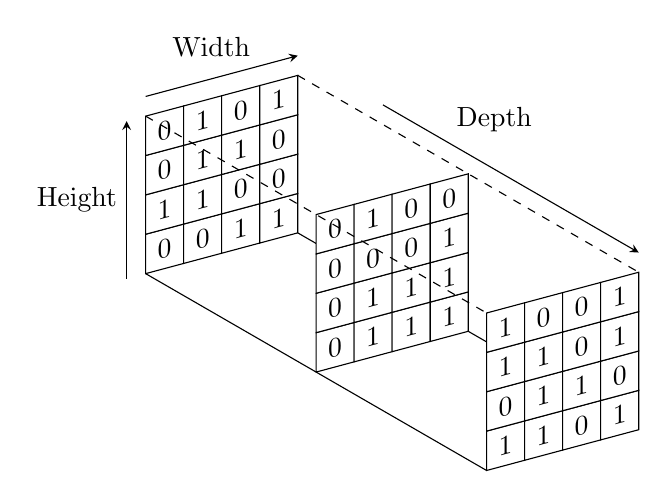
\begin{tikzpicture}[x=(15:.5cm), y=(90:.5cm), z=(330:.5cm), >=stealth]
\draw (0, 0, 0) -- (0, 0, 10) (4, 0, 0) -- (4, 0, 10);
\foreach \z in {0, 5, 10} \foreach \x in {0,...,3}
  \foreach \y [evaluate={\b=random(0, 1);}] in {0,...,3}
    \filldraw [fill=white] (\x, \y, \z) -- (\x+1, \y, \z) -- (\x+1, \y+1, \z) --
      (\x, \y+1, \z) -- cycle (\x+.5, \y+.5, \z) node [yslant=tan(15)] {\b};
\draw [dashed] (0, 4, 0) -- (0, 4, 10) (4, 4, 0) -- (4, 4, 10);
\draw [->] (0, 4.5, 0)  -- (4, 4.5, 0)   node [near end, above left] {Width};
\draw [<-] (-.5, 4, 0)  -- (-.5, 0, 0)   node [midway, left] {Height};
\draw [<-] (4, 4.5, 10) -- (4, 4.5, 2.5) node [near end, above right] {Depth};
\end{tikzpicture}%
\end{center}

\end{frame}
\subsection{Explaining the Mathematics}
\begin{frame}
  \frametitle{Explaining the Mathematics}
\end{frame}
\subsection{Theoretical Complexity}
\begin{frame}
  \frametitle{Theoretical Complexity}
\end{frame}
\subsection{Experimental Analysis}
\begin{frame}
  \frametitle{Experimental Analysis}
\end{frame}
\subsection{Results}
\begin{frame}
  \frametitle{Results}
\end{frame}

%%%%%%%%%%% SECTION 2%%%%%%%%%%%%%%%
% \section{Euclidean Distance Reduction}

% \subsection{General Idea}
% \begin{frame}
%   \frametitle{General Idea}
% \end{frame}
% \subsection{Explaining the Mathematics}
% \begin{frame}
%   \frametitle{Explaining the Mathematics}
% \end{frame}
% \subsection{Theoretical Complexity}
% \begin{frame}
%   \frametitle{Theoretical Complexity}
% \end{frame}
% \subsection{Experimental Analysis}
% \begin{frame}
%   \frametitle{Experimental Analysis}
% \end{frame}
% \subsection{Results}
% \begin{frame}
%   \frametitle{Results}
% \end{frame}

%%%%%%%%%%% SECTION 3%%%%%%%%%%%%%%%

\section{Compression via k-d Tree}
%%%%%%%%%%% SECTION 3%%%%%%%%%%%%%%%
\subsection{General Idea}
\begin{frame}
  \frametitle{General Idea}
\end{frame}
\subsection{Explaining the Mathematics}
\begin{frame}
  \frametitle{Explaining the Mathematics}
\end{frame}
\subsection{Theoretical Complexity}
\begin{frame}
  \frametitle{Theoretical Complexity}
\begin{itemize}
\item Insertion time for a K-d tree is $O (\log(n))$
\item Any traversal is $O(n+m)$, where $m$ is the number of edges
\item $m = K n$ as each node can have $K$ children, this simplifies the traversal time to 
$$O(n+kn)$$
\item Since $k$ is a constant, $O(n(k+1)) = O(n)$
\item Hence the cost of traversal becomes $$O(n)$$
    
\end{itemize}
\end{frame}
\subsection{Experimental Analysis}
\begin{frame}
  \frametitle{Experimental Analysis}
\end{frame}
\subsection{Results}
\begin{frame}
  \frametitle{Results}
\end{frame}




% All of the following is optional and typically not needed. 
\appendix
\section<presentation>*{\appendixname}
\subsection<presentation>*{Bibliography}

\begin{frame}[allowframebreaks]
  \frametitle<presentation>{For Further Reading}
    
  \begin{thebibliography}{10}
    
  \beamertemplatebookbibitems
  % Start with overview books.

  \bibitem{Author1990}
    A.~Author.
    \newblock {\em Handbook of Everything}.
    \newblock Some Press, 1990.
 
    
  \beamertemplatearticlebibitems
  % Followed by interesting articles. Keep the list short. 

  \bibitem{Someone2000}
    S.~Someone.
    \newblock On this and that.
    \newblock {\em Journal of This and That}, 2(1):50--100,
    2000.
  \end{thebibliography}
\end{frame}


\end{document}


